\documentclass[a4paper,12pt]{article}
\usepackage[utf8]{inputenc}
\usepackage{graphicx}
\usepackage{amsmath}
\usepackage{hyperref}
\usepackage{enumitem}
\usepackage{geometry}
\usepackage{fancyhdr}
\usepackage{titlesec}
\usepackage{tabularx}
\usepackage{float}
\usepackage{xcolor}
\usepackage{booktabs}
\usepackage{tablefootnote}
\usepackage{adjustbox}
\usepackage{fancyhdr}
\usepackage{url}
\usepackage{cite}

\geometry{margin=1in}
\fancyhf{}
\rfoot{\thepage}

\titleformat{\section}{\Large\bfseries}{\thesection}{1em}{}
\titleformat{\subsection}{\large\bfseries}{\thesubsection}{1em}{}

\title{Relatório do Projeto: 1ª Versão}
\date{\today}

\geometry{top=1in, bottom=1in, left=1.25in, right=1in}

\pagenumbering{arabic}

\begin{document}

\begin{center}
    \large\textbf{UNIVERSIDADE DE AVEIRO} \\[1.5cm]
    
    
\includegraphics[width=10cm]{images/Universidade-de-Aveiro.png} \\[1.5cm]
    
    \Huge \textbf{Técnicas de Mineração\\ de Texto - 2} \\[1.5cm]

    \normalsize Licenciatura em Engenharia de Computadores e Informatica \\[0.5cm]
    UC: Projeto em Engenharia de Computadores e Informática \\[0.5cm]
    \textbf{Membros do Grupo:} Gabriel Boia (113167), Guilherme Matos (114252), Rafael Dias (114258), Tiago Costa (114629) e Tiago Almeida (113106) \\[0.5cm]
    \textbf{Professor Coordenador:} Luís Filipe de Seabra Lopes \\[2cm]
    \vfill
    \textbf{\today} \\[1cm]
\end{center}
\newpage

\newpage
% \maketitle
\tableofcontents
\newpage

\section{Abstract}
Empresas que trabalham com grandes volumes de dados devem manter um padrão definido, de modo a garantir um acesso à informação rápido e eficaz. A proposta deste projeto surgiu de uma necessidade real da Administração dos Portos de Sines e do Algarve, S.A., que tem vindo a enfrentar cada vez mais dificuldades na gestão estatística dos dados face às diversas variações de nomes de empresas que surgem nos seus registos. Este projeto insere-se também no âmbito do projeto NEXUS\footnote{NEXUS: Pacto de Inovação – Transição Verde e Digital para Transportes, Logística e Mobilidade}.
\\
O grupo descreve no presente relatório o trabalho realizado no sentido de desenvolver um método automático para a correção e padronização destes nomes, com base na associação de colunas entre tabelas, técnicas de comparação textual e de agrupamento não supervisionado e semi-supervisionado. O sistema recebe como entrada as tabelas de dados a corrigir e, opcionalmente, uma tabela de dados de referência com os nomes e informação padronizada de cada empresa.

\section{Introdução}
\subsection{Contexto}

Dado um conjunto de dados no qual grande parte da informação em cada linha é escrita de forma livre, isto é, sem restrições sobre o método de introdução de dados, é natural que ocorram inconsistências, erros de digitação ou falta de padronização. No contexto específico deste projeto, os conjuntos de dados dizem respeito às empresas que entram e saem do Porto de Sines \footnote{Todos os conjuntos de dados foram fornecidos pelo Porto de Sines sob um contrato de confidencialidade.}.

Como os registos das empresas são efetuados manualmente, é comum que uma mesma entidade surja com variações no nome (por exemplo, diferenças de acentuação ou espaçamento irregular). Essa problemática estende-se também a outros campos, como números de identificação (NIF).

Partindo da existência de uma base de dados de referência contendo os nomes padronizados e a informação fidedigna de cada empresa, é possível proceder à correção automática de grande parte dos dados originais, reduzindo significativamente o esforço de correção manual.

Para identificar e agrupar nomes semelhantes, o sistema desenvolvido recorre a diversas métricas de comparação textual, tanto de similaridade quanto de distância. Entre as principais métricas utilizadas encontram-se a distância de Levenshtein, que quantifica o número mínimo de operações de edição necessárias para transformar uma cadeia de caracteres noutra; o índice de Jaccard, uma métrica de similaridade baseada na interseção e união de conjuntos de caracteres (sendo a distância de Jaccard definida como \(1 - J\)); e a similaridade de cosseno, geralmente aplicada a vetores de frequência ou representações vetoriais de texto.

Além disso, foi utilizado um modelo de linguagem para vetorização semântica das palavras, tornando a comparação mais robusta. Todas estas técnicas foram integradas num algoritmo de agrupamento (\textit{clustering}), que agrupa variantes semelhantes de nomes e sugere a forma padronizada, seja esta proveniente da tabela de referência ou inferida com base nos dados disponíveis.


\subsection{Objetivos}
O objetivo do projeto desenvolvido incide na criação de um sistema que tem como finalidade principal corrigir e padronizar grandes bases de dados. É de realçar que a solução desenvolvida requer a existência dos campos de nome e número de identificação para o seu funcionamento, dado que estas foram as informações usadas no seu desenvolvimento.
\\
Para que o sistema funcione podem ser introduzidos dois tipos de conjuntos de dados:
\begin{enumerate}
    \item Um ou mais conjuntos de dados a corrigir (Obrigatório)
    \item Um ou mais conjuntos de dados que incluam as informações padronizadas de cada empresa (Opcional)
\end{enumerate}
Apesar do sistema desenvolvido ter a possibilidade de operar sem uma tabela de dados de referência, a sua existência leva a resultados melhores, explorados com maior detalhe em \ref{testes}.

\subsection{Enquadramento Académico}
Este trabalho foi realizado ao longo do ano letivo 2024/2025, no âmbito da unidade curricular de PECI (Projeto em Engenharia de Computadores e Informática), sob supervisão do professor Luís Seabra Lopes e acompanhamento dos docentes responsáveis.

\section{Requisitos}
Nesta secção, é abordada a escolha dos \textit{stakeholders} envolvidos no projeto, e são reconhecidos os requisitos e métodos de recolha dos mesmos, bem como a importância individual de cada um.

\subsection{Análise dos \textit{Stakeholders}}
Tendo em mente o objetivo fundamental do projeto, é possível identificar três \textit{stakeholders}:
\begin{enumerate}
    \item Todos os membros do grupo, como desenvolvedores do sistema;
    \item O professor orientador do projeto (Prof. Luís Seabra Lopes);
    \item A empresa que submete a proposta do projeto:  Administração dos Portos de Sines e do Algarve, S.A.
\end{enumerate}

\subsection{Métodos de Recolha de Requisitos}
Após a definição dos \textit{stakeholders}, foram levantados os requisitos relativos ao projeto.
\\
Para tal, o grupo fez uso de métodos diferentes:
\begin{enumerate}
    \item Contacto direto com a empresa interessada, por intermediário do professor orientador
    \item Reuniões entre os desenvolvedores
    \item Discussão com os professores responsáveis pela Unidade Curricular
\end{enumerate}

\subsubsection{Contacto direto com a empresa interessada}
A partir do contacto com o Porto de Sines, nomeadamente através de reuniões com o professor orientador, o grupo estabeleceu os requisitos mais importantes, que definem o objetivo do trabalho e que foram considerados fundamentais para o sucesso do projeto.

\subsubsection{Reuniões entre os desenvolvedores}
Através de reuniões internas, obteve-se uma perspetiva de como seria possível alcançar os requisitos mais importantes e definiram-se ainda requisitos secundários que o grupo sentiu que trariam mais valor ao projeto sem comprometer a realização dos requisitos principais.

\subsubsection{\textit{Feedback} dos professores responsáveis pela UC}
Por último, as aulas da Unidade Curricular associada ao projeto, mais especificamente as aulas onde houve um contacto mais direto com os professores responsáveis, permitiram uma solidificação das ideias previamente discutidas em grupo e também trouxeram novas ideias e pontos de vista úteis ao desenvolvimento do trabalho.

\subsection{Requisitos Definidos}
Uma vez que explicados os métodos de levantamento de requisitos, apresentam-se de seguida os requisitos definidos em última análise, juntamente com a sua classificação (funcional ou não funcional. Adicionalmente, na tabela também se encontra a referência à completude do requisito aquando da entrega do projeto. Os requisitos encontram-se divididos em duas tabelas (\ref{tab:requirements} e \ref{tab:requirements-secondary}), de acordo com a sua prioridade no contexto do projeto. Os requisitos principais distinguem-se por serem fundamentais para o sucesso do projeto, enquanto que os requisitos secundários foram encarados como \textit{extras} que dariam um valor maior ao projeto.

\subsubsection{Requisitos Principais}
\begin{table}[h!]
    \centering
    \begin{tabularx}{\textwidth}{|X|l|c|}
        \hline
        \textbf{Descrição do Requisito} & \textbf{Tipo} & \textbf{Atingido} \\ \hline
        Corrigir os dados & Funcional & Sim \\ \hline
        Assegurar precisão na correção & Não Funcional & Sim \\ \hline
        Adaptável (capaz de trabalhar com diferentes \textit{datasets}) & Funcional & Sim\\ \hline
        Reduzir significativamente o trabalho manual de correção posterior & Funcional & Sim\\ \hline
    \end{tabularx}
    \caption{Resumo dos Requisitos Principais}
    \label{tab:requirements}
\end{table}
\subsubsection{Requisitos Secundários}
\begin{table}[h!]
    \centering
    \begin{tabularx}{\textwidth}{|X|l|c|}
        \hline
        \textbf{Descrição do Requisito} & \textbf{Tipo} & \textbf{Realizado} \\ \hline
        Baixa complexidade temporal & Não Funcional & Sim \\ \hline
        Inserir novas entradas nos dados padronizados (quando surgem novas empresas) & Funcional & Não \\ \hline
        Capacidade de sugerir entradas quando alguém insere uma entrada que se assemelhe a um campo padronizado & Funcional & Não \\ \hline
        Ter uma \textit{User Interface} de forma a poder interagir com o programa de forma fácil & Não Funcional & Sim (interface no terminal)\\ \hline
    \end{tabularx}
    \caption{Resumo dos Requisitos Secundários}
    \label{tab:requirements-secondary}
\end{table}

\newpage
\section{\textit{Background} e Trabalhos Relacionados}
% \subsection{Contextualização do Problema}
% Este projeto insere-se na área de Ciência de Dados, mais concretamente no âmbito de \textit{limpeza de dados} (data cleansing), uma etapa fundamental na preparação dos dados para a sua análise e tratamento. No contexto específico deste trabalho, que decorre no âmbito do projeto \textbf{NEXUS}, o foco está na padronização de dados reais relativos a uma empresa. Esta padronização é crucial para garantir a integridade dos dados registados no sistema do porto, bem como para facilitar a sua gestão e análise posterior.
% \\
% Uma das maiores dificuldades enfrentadas neste processo é o tratamento de conjuntos de dados de grande dimensão, muitos dos quais se encontram fora dos padrões de registo esperados e contêm erros ortográficos. Por exemplo, é comum encontrar campos com abreviações de nomes de empresas ou até mesmo com sinais de pontuação indesejados no início, meio ou fim das \textit{strings}.

\subsection{Soluções Existentes}
Numa pesquisa inicial, o grupo teve a preocupação de procurar trabalhos e técnicas de limpeza de dados que fossem relevantes ao problema em mãos, de modo a facilitar a recolha de dados inicial, bem como o levantamento de técnicas que poderiam ser aplicadas na resolução do problema. Foram assim encontrados dois projetos considerados relevantes:

\begin{enumerate}
    \item \textbf{SymSpell Algorithm}\cite{symspell2025}:
    Este projeto oferece uma abordagem eficiente para a correção de frases e palavras relativamente curtas, preparada para lidar com grandes volumes de dados. O trabalho tem por base o \textit{Symmetric Delete Algorithm}. Este algoritmo reduz a complexidade do problema ao gerar variações mínimas de cada frase, de modo a simular possíveis erros ortográficos que possam ser cometidos.\\
    Isto passa pela remoção ou adição de certos caracteres à palavra, ou até mesmo a troca de caracteres adjacentes. Estas variações são então procuradas nas chaves de um dicionário de correspondência, que tem como valor de cada chave a frase correta. Caso seja obtida mais do que uma correspondência, é então calculada a distância de Levenshtein da frase original ao valor da correspondência obtida, de modo a verificar qual a frase pretendida (sendo possível mais do que uma correspondência legítima). Não sendo obtidos resultados diretos, ou a palavra não é corrigida, ou é feita uma procura mais profunda com a distância de Levenshtein.

    \item \textbf{CPClean}\cite{cpclean2021}:
    Este projeto, menos notório que o supracitado, passa por uma estratégia que tem como objetivo a limpeza dos dados pretendidos, de modo a melhorar a exatidão de modelos de correção através de Aprendizagem Automática. Assim, o seu objetivo não é a correção direta dos campos de dados, mas sim a sua limpeza e preparação que auxilia na correção feita posteriormente.
\end{enumerate}

\subsection{Inovação e diferenciação}

Apesar da relevância de ambos os projetos, estes têm as suas limitações e problemas, quer no seu todo, quer no contexto do atual projeto. \\
Uma limitação do \textbf{SymSpell Algorithm} passa pelo facto de estar projetado para lidar com palavras ou frases de dimensões reduzidas, que não é o caso com o tipo de dados a corrigir. Também o facto deste algoritmo ser projetado para lidar com pequenas variações previsíveis nas frases ou palavras o torna mais difícil de aplicar no contexto do projeto atual, visto que as variações que surgem dos nomes de empresas são muitas vezes constituídas por erros imprevisíveis e de grande dimensão, com muitas palavras a mais ou em falta.
\\
Em relação ao \textbf{CPClean}, um dos seus maiores problemas é a escassez de documentação do projeto. 
\\
%new
No entanto, ainda que relevantes, os projetos mencionados foram utilizados apenas como repositórios de técnicas de análise e comparação de palavras ou frases, como as distâncias de Levenshtein e a utilização de dicionários de correspondências, que proporcionou a redução dos tempos de resolução de campos de dados que já tenham sido resolvidos anteriormente.
% Para além disso, o grupo decidiu afastar-se, numa fase inicial, de métodos que façam uso direto de \textit{machine learning} para correção dos campos de dados, ainda que não excluindo esta alternativa de resolução. Este afastamento veio do feedback dos professores da Unidade Curricular, aquando do início da exploração do tema. \\
% No entanto, conseguiu-se retirar destes projetos conhecimentos úteis para a correção dos campos de dados, como o uso das distâncias de Levenshtein e a utilização de um dicionário de correspondências com a intenção de reduzir os tempos de resolução de campos de dados com erros que já tenham sido vistos/resolvidos anteriormente.

\section{Design e Soluções Viáveis}
\subsection{Design do Sistema}

O sistema desenvolvido para validar e corrigir nomes baseia-se em dois componentes principais:
\begin{itemize}
    \item \textbf{Tabelas a serem corrigidas}: Contém os nomes que necessitam de validação e padronização. (Obrigatório)
    \item \textbf{Tabelas referência (Standard)}: Conjunto de nomes previamente validados, utilizados como referência, caso as tabelas sejam introduzidas. (Opcional)
    %\item \textbf{Dicionário de sinónimos}: Estrutura que armazena associações conhecidas entre nomes alternativos e os seus correspondentes padrão.%
\end{itemize}
%new
O sistema recebe como entrada a(s) tabela(s) mencionada(s). Os nomes das empresas são extraídos de cada tabela e processados com o objetivo de realizar uma limpeza, removendo ruído indesejável. Opcionalmente, o utilizador pode fornecer uma tabela de referência, a partir da qual é construída uma base de verdade (\textit{Ground Truth}) para avaliar o desempenho do algoritmo de agrupamento. Esta base de verdade é formada agrupando os nomes das empresas que partilham o mesmo número de identificação na tabela de referência. Caso esta tabela não seja fornecida, não é criada qualquer base de verdade, e o agrupamento prossegue sem validação automática.
\\
Os nomes a corrigir são convertidos em vetores semânticos utilizando o módulo Python \textit{SentenceTransformers}\footnote{\url{https://sbert.net/}}. Estes vetores são normalizados e indexados com recurso à biblioteca \textbf{FAISS} \footnote{\url{https://faiss.ai/index.html}} - explorada em detalhe em \ref{faiss} - permitindo comparações rápidas e eficientes entre nomes com base na sua similaridade vetorial.
%old
% O sistema recebe como entrada uma lista de nomes, que depois serão limpos, e opcionalmente recebe \textit{tabela standard}, usada para criar a groundtruth (grupos de nomes já associados entre si). Estes nomes são então convertidos em vetores semânticos utilizando \textit{sentence embeddings}. Os vetores gerados são normalizados e indexados com recurso à biblioteca do FaceBook, FAISS, explorada em detalhe na secção que se segue, permitindo comparações rápidas e eficientes entre nomes com base na sua similaridade vetorial.
\\
O fluxo do algoritmo de agrupamento é ilustrado na Figura \ref{fig:design} e segue os seguintes passos principais:

\begin{enumerate}
    \item \textbf{Criação de um novo grupo}: Para cada nome ainda não associado, é criado inicialmente um novo grupo com esse nome.

    \item \textbf{Procura de nomes semelhantes}: O sistema utiliza a biblioteca \textbf{FAISS} para identificar os 1000 nomes semânticamente mais semelhantes com base nos vetores indexados. Estes 1000 nomes podem originar dos nomes a analisar ou dos nomes já tidos no agrupamento. Para cada nome candidato, é calculada a similaridade com o nome a ser atualmente analisado.

    \item \textbf{Atribuição a grupos}: Se a similaridade entre o nome atual e os candidatos for acima de um limiar definido, estes são agrupados ao grupo criado (mencionado no primeiro ponto). Caso o nome semelhante já pertença a um grupo originado a partir da base de verdade, o seu index é guardado, bem como o valor da sua similaridade, como um possível \textit{best match}. No final da comparação com todos os nomes, o novo grupo criado vai extender o grupo do seu \textit{best match} ou, caso não tenha sido encontrado um, vai ser anexado no final do agrupamento como um novo grupo distinto. É relevante mencionar que nos nomes inseridos no conjunto de dados sobre o qual se trabalhou, muitas das entradas referentes ao nome da empresa incluíam nomes pessoais (possivelmente por serem referentes a empresas familiares). Para isso, o grupo criou uma regra que reconhece se a entrada é um nome e, caso positivo, aumenta o limiar de similaridade de forma a que os nomes só entrem no mesmo grupo caso sejam realmente semelhantes. A necessidade para esta correção surge porque os vetores gerados para nomes de pessoas são sempre relativamente semelhantes, por serem semânticamente parecidos.

    \item \textbf{Novo ciclo}: Os nomes que foram anexados são marcados como vistos para serem ignorados em futuras iterações, e isto repete-se para cada nome a ser analisado.
\end{enumerate}

\begin{figure}[H]
    \centering
    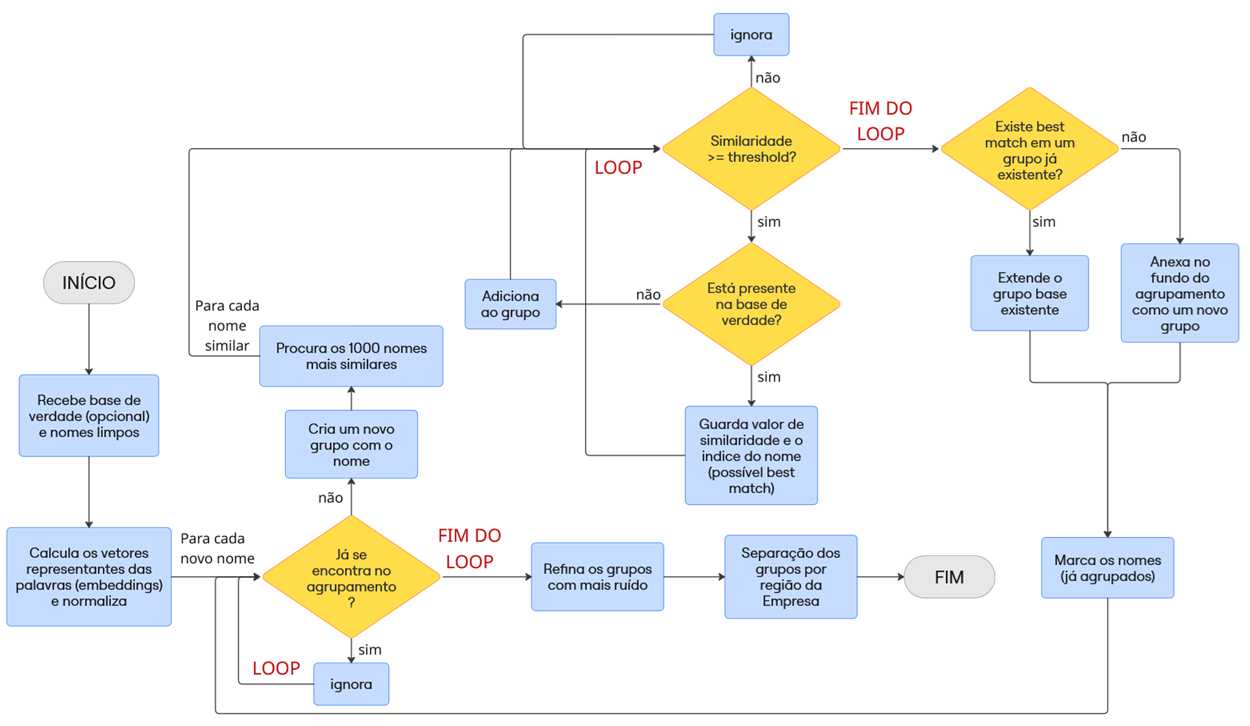
\includegraphics[width=0.8\textwidth]{images/ClusteringFluxogram.png}
    \caption{Fluxo do Sistema de Agrupamento}
    \label{fig:design}
\end{figure}

\subsection*{Pseudocodigo do Algoritmo}

\noindent\textbf{Entradas:}
\begin{itemize}
    \item \texttt{BASE}: lista de listas de nomes associados, ex. \texttt{[[N1a, N1b, ...], [N2a, N2b, ...]]}
    \item \texttt{AGRUPAR}: lista de nomes únicos a agrupar
\end{itemize}

\vspace{0.5em}
\noindent\textbf{Inicialização:}
\begin{enumerate}
    \item Criar \texttt{MAPA} $\leftarrow$ dicionário \{nome $\rightarrow$ índice do grupo em \texttt{BASE}\}
    \item \texttt{NOMES} $\leftarrow$ todos os nomes presentes em \texttt{BASE} e \texttt{AGRUPAR}
    \item \texttt{VECTORES} $\leftarrow$ vetores semânticos de \texttt{NOMES} com \textit{SentenceTransformer}
    \item \texttt{GRUPOS} $\leftarrow$ cópia de \texttt{BASE}
    \item \texttt{AGRUPADOS} $\leftarrow$ Verdadeiro para n em \texttt{NOMES} se n existe em \texttt{GRUPOS} caso contrário Falso 
\end{enumerate}

\vspace{0.5em}
\noindent\textbf{Para cada nome $n$ em \texttt{NOMES}:}
\begin{enumerate}
    \item[1.] Se \texttt{AGRUPADOS[indice(Nomes,$n$)]} == Verdadeiro, continuar para o próximo nome
    \item[2.] \texttt{NOVO} $\leftarrow$ \{ $n$ \}
    \item[3.] \texttt{CANDIDATOS} $\leftarrow$ 1000 nomes mais semelhantes a $n$ em \texttt{VECTORES}, retorna (índice, similaridade)
    \item[4.] \texttt{maxMatch} $\leftarrow$ 0;\quad \texttt{bestMatch} $\leftarrow$ \texttt{None}
    \item[5.] Para cada $(i, s)$ em \texttt{CANDIDATOS}:
    \begin{enumerate}
        \item[a.] Se $s <$ \texttt{threshold}, continuar para o próximo
        \item[b.] Se \texttt{NOMES[$i$]} $\in$ \texttt{MAPA} (ou seja, está na base de verdade):
        \begin{itemize}
            \item Se $s >$ \texttt{maxMatch}, então:
            \begin{itemize}
                \item \texttt{maxMatch} $\leftarrow s$
                \item \texttt{bestMatch} $\leftarrow$ \texttt{MAPA[NOMES[$i$]]}
            \end{itemize}
        \end{itemize}
        \item[c.] Caso contrário:
        \begin{itemize}
            \item Adicionar \texttt{NOMES[$i$]} a \texttt{NOVO}
            \item \texttt{AGRUPADOS[$i$]} $\leftarrow$ Verdadeiro
        \end{itemize}
    \end{enumerate}
    \item[6.] Se \texttt{bestMatch} == \texttt{None}:
    \begin{itemize}
        \item Adicionar \texttt{NOVO} a \texttt{GRUPOS}
    \end{itemize}
    \item[7.] Caso contrário:
    \begin{itemize}
        \item Adicionar \texttt{NOVO} ao grupo \texttt{GRUPOS[bestMatch]}
    \end{itemize}
\end{enumerate}

\vspace{0.5em}
\noindent\textbf{Pós-processamento:}
\begin{itemize}
    \item Refinamento de grupos com maior ruído
    \item Eventual separação adicional por região geográfica
\end{itemize}

\vspace{0.5em}
\noindent\textbf{Retorna:} \texttt{GRUPOS}

\subsection{Pós-processamento:}
\begin{itemize}
    \item \textbf{Deteção e remoção de ruído:}
    \begin{itemize}
        \item Para os grupos com maior número de elementos, calcular a média de similaridade entre os seus membros.
        \item Identificar elementos cuja similaridade com os restantes do grupo seja significativamente inferior à média.
        \item Esses elementos são movidos para um novo grupo individual (tratados como possíveis outliers).
    \end{itemize}
    
    \item \textbf{Separação por região geográfica:}
    \begin{itemize}
        \item Para cada grupo, verificar se os nomes associados pertencem a diferentes países (inferência por nome).
    \end{itemize}
\end{itemize}

\subsection{Remoção de Ruído em Clusters}

Para reduzir o ruído presente nalguns clusters resultantes da fase de agrupamento, aplicou-se um processo de \textit{refinamento de grupos}. Este processo visa identificar nomes que, apesar de inicialmente agrupados juntos, apresentam uma similaridade significativamente inferior com os restantes elementos do cluster.

\vspace{0.5em}
\noindent A metodologia baseia-se numa métrica de similaridade combinada, definida da seguinte forma:

\begin{itemize}
    \item \textbf{Similaridade de Levenshtein Normalizada:} Calcula a distância de Levenshtein entre os nomes, após remoção de prefixos legais (e.g., "Sociedade", "Empresa") e termos geográficos (e.g., "Brasil", "Angola"). A similaridade é então dada por $1 - \frac{\text{distância}}{\text{comprimento máximo}}$.
    
    \item \textbf{Jaccard Ponderado:} Baseado no índice de Jaccard entre os tokens dos nomes. Tokens considerados genéricos (prefixos legais e regiões) são ignorados na interseção. A interseção ponderada considera apenas tokens distintos e relevantes.
    
    \item \textbf{Combinação Final:} A similaridade final entre dois nomes é uma média ponderada: 
    \[
    \text{similaridade}(n_1, n_2) = 0{,}7 \cdot \text{Levenshtein}(n_1, n_2) + 0{,}3 \cdot \text{Jaccard}(n_1, n_2)
    \]
\end{itemize}

\vspace{0.5em}
\noindent O algoritmo percorre os elementos de um cluster inicial e reagrupa os nomes em subconjuntos onde todos os pares de nomes possuem uma similaridade combinada superior a $0{,}75$. Caso um nome não atinja esse limiar com nenhum grupo existente, é colocado num novo grupo.


\noindent Este processo permite reduzir significativamente o ruído, isolando nomes que foram agrupados de forma incorreta devido a coincidências superficiais.


\subsection{Biblioteca FAISS} \label{faiss}

\textbf{FAISS} (\textit{Facebook AI Similarity Search}) é uma biblioteca desenvolvida pelo Facebook AI Research\footnote{Agora Meta Research} que permite a realização de pesquisas eficientes de vetores em espaços de alta dimensão. Foi desenhada para escalar a tarefas de busca aproximada por similaridade, com foco em desempenho e precisão, sendo amplamente utilizada em aplicações de recuperação de informação, recomendação e agrupamento semântico.
\\
No contexto deste sistema, \textbf{FAISS} é utilizada para identificar rapidamente nomes semanticamente semelhantes através das seguintes funcionalidades principais:

\begin{itemize}
    \item \textbf{Normalização de vetores}: Após a geração dos vetores semânticos (através de \textit{sentence embeddings} criados com \textit{SentenceTransformers}), os vetores são normalizados com \textbf{FAISS} para que a métrica de similaridade baseada em produto interno (\textit{inner product}) funcione de forma equivalente à distância de cosseno.

    \item \textbf{Indexação eficiente}: Os vetores são armazenados num índice \textbf{FAISS}, permitindo consultas extremamente rápidas mesmo com milhares de nomes.

    \item \textbf{Pesquisa por similaridade}: \textbf{FAISS} permite encontrar os $k$ vetores mais próximos de um dado vetor de entrada, retornando os índices e os valores de similaridade correspondentes. Esta funcionalidade é essencial para agrupar nomes com base na proximidade semântica.

\end{itemize}
A utilização da biblioteca \textbf{FAISS} permitiu uma redução significativa no tempo de execução e uma maior escalabilidade do sistema, especialmente quando aplicado a volumes muito grandes de dados.

\subsection{Soluções Alternativas}

Durante a evolução do projeto, outras soluções foram consideradas e testadas, pelo que são aqui explorados os aspetos positivos e negativos levantados com o uso destas soluções:

\label{sec:MinHash}
\begin{enumerate}
    \item \textbf{Distância de Levenshtein como única técnica}  
    \begin{itemize}
        \item \textbf{Vantagem}: Simplicidade na implementação, já que todas as entradas seriam corrigidas com base na proximidade.
        \item \textbf{Desvantagem}: Não é considerada a semântica dos nomes, o que pode levar a agrupamentos incorretos. Além disso, erros comuns ou abreviações podem não ser corrigidos de forma adequada.
    \end{itemize}
    
    \item \textbf{Uso de Machine learning}  
    \begin{itemize}
        \item \textbf{Vantagem}: Um modelo treinado poderia identificar padrões de erros mais complexos, aprendendo a corrigir mesmo entradas fora do comum.
        \item \textbf{Desvantagem}: Requer uma grande quantidade de dados curados e tempo de treino. Além disso, devido à escassez desses dados neste contexto, a utilização de \textit{Machine Learning} seria menos eficaz do que abordagens baseadas em regras e similaridade textual.
    \end{itemize}
    
    \item \textbf{Criação de um dicionário manual}  
    \begin{itemize}
        \item \textbf{Vantagem}: Total controlo sobre as correções.
        \item \textbf{Desvantagens}: Processo manual e inviável para grandes volumes de dados. Impossibilidade de prever todas as variações, dada a elevada imprevisibilidade.
    \end{itemize}

    \item \textbf{Uso de MinHash com Similaridade de Jaccard}  
    \begin{itemize}
        \item \textbf{Vantagem}: Permite calcular a similaridade entre nomes com base na sobreposição de substrings (shingles), sendo extremamente eficiente para detectar pequenas variações ortográficas.
        \item \textbf{Desvantagem}: Pode não capturar bem relações semânticas entre palavras. A performance depende da escolha de parâmetros, como por exemplo o número de funções \textit{hash}. Esta abordagem revelou ser substancialmente mais lenta que a abordagem final, com \textit{SentenceTransformers} e \textbf{FAISS}.
    \end{itemize}
\end{enumerate}

% \subsection{Solução escolhida}

% Em última análise, optou-se pela combinação do dicionário JSON com a métrica de distância de Levenshtein por diversos motivos:  
% \begin{itemize}
%     \item \textbf{Eficiência}: Correções rápidas para nomes já conhecidos, reduzindo a necessidade de cálculos repetidos.
%     \item \textbf{Adaptabilidade}: O sistema está a ser melhorado continuamente à medida que novas associações são registadas no JSON.
%     \item \textbf{Facilidade de revisão}: Entradas não resolvidas são organizadas para análise manual, garantindo precisão.
% \end{itemize}

% Esta abordagem equilibra eficiência automatizada e controlo manual, atendendo aos requisitos do projeto e garantindo um sistema flexível e preciso para validação de nomes.



\subsection{Solução Final}

A solução adotada baseia-se na utilização de algoritmos de agrupamento, para agrupar as entradas semelhantes no campo referente ao nome da empresa. Através desta abordagem, é possível identificar e consolidar variações do mesmo nome, mesmo quando contêm erros ortográficos, abreviações ou formatos distintos.
\\
Para isso, é realizada inicialmente um pré-processamento dos nomes, onde cada entrada é normalizada com base em regras definidas - remoção de pontuação, passagem a letras minúsculas, entre outros. Após essa etapa, são extraídas representações vetoriais dos nomes, de modo a permitir a comparação mais eficaz entre nomes.
\\
Posteriormente, é aplicado um algoritmo de agrupamento com um limiar de semelhança adequado, de forma a garantir que apenas nomes suficientemente semelhantes são agrupados. Cada grupo resultante sem entrada na tabela de referência é então associado a um nome tido como nome representante do grupo, selecionado com base na entrada mais próxima do centro do próprio grupo.
\\
Esta abordagem tem como vantagem principal a sua capacidade de lidar com variações imprevisíveis nos dados, sem depender de um dicionário fixo de nomes. Além disso, permite escalar a limpeza a conjuntos de dados de grandes dimensões, adaptando-se dinamicamente às entradas presentes.
\\
Todo este sistema funciona em conjunto com uma interface de terminal simples que permite a escolha dos ficheiros a serem introduzidos, bem como a visualização do progresso do programa. A interface dá ainda a escolher ao utilizador se este pretende receber informação relativa à avaliação da precisão da correção realizada sobre os dados.

% \section{Desenvolvimento atual}
% \subsection{Progresso}
% O projeto atualmente encontra-se na sua fase mais crucial e trabalhosa, tal como o nome do projeto sugere a mineração de texto incorpora um papel importante no desenvolvimento deste projeto, com o objetivo de conseguir criar um sistema para a standardização das bases de dados do Porto de Sines é importante que tenhamos a certeza de que os valores que estamos a utilizar para a standardização estão corretos, neste momento o projeto encontra-se numa fase em que estamos focados em fazer uma associação correta entre os dados corretos e os dados incorretos, para este fim estamos a utilizar uma técnica para cálculo de diferênças entre strings, a distância de Levenshtein, criada em 1965 por Vladimir Levenshtein. O nosso objetivo para o futuro seria com esta técnica conseguir criar um dicionário em que temos os nomes incorretos como chave e os nomes corretos como valor para consulta e correção eficiente dos dados.

% \subsection{Demonstração}
% A demonstração do nosso projeto é feita em python já que contem disponivéis várias bibliotecas que facilitam a manipulação de dados.
% Apesar de não demonstrar todas as capacidades que tencionamos que existam no final do projeto, já apresenta o fundamental.
% A demonstração foi feita num ambiente bastante controlado já que a quantidade de dados corretos que temos para utilizar é pequena.
% Lê o ficheiro onde está guardado o dicionário com os nomes incorretos associados aos nomes corretos.
% \vspace{0.5cm}

% 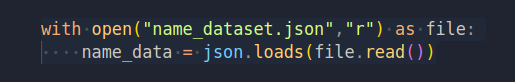
\includegraphics[width=14cm]{images/Screenshot1.png} \\[0.5cm]
% Por cada nome existente no dataset procura as linhas do dataset onde o nome é igual e também procura na tabela de dados standardizados a linha correspondente à correção desse nome.
% Se o nome não existir no dicionário de nomes é adicionado á lista de nomes desconhecidos.
% Se o nome existir no dicionário de nomes, substitiu todas as linhas com esse nome para os valores corretos presentes no dataset standard.
% \vspace{0.5cm}

% 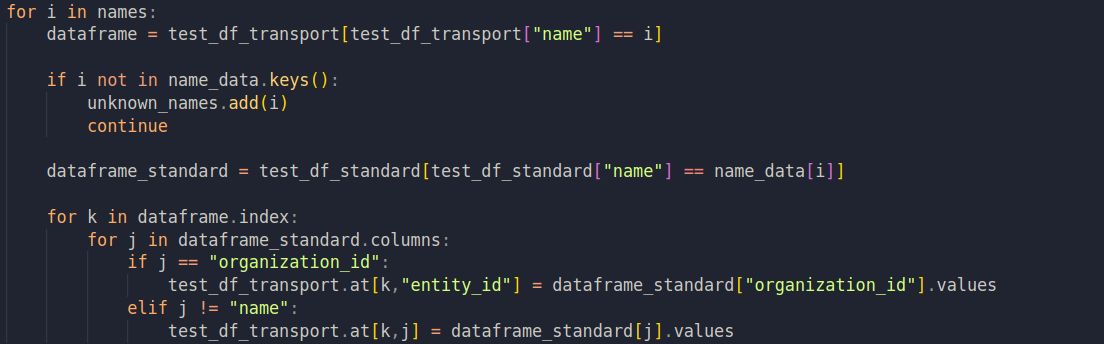
\includegraphics[width=14cm]{images/Screenshot2.png} \\[0.5cm]
% Para cada nome desconhecido devolve uma lista com os nomes standard mais próximos e pergunta ao utilizador se pretendia referir-se a algum deles. Se sim uma nova entrada é adicionada ao dicionário de nomes conhecidos.
% \vspace{0.5cm}

% 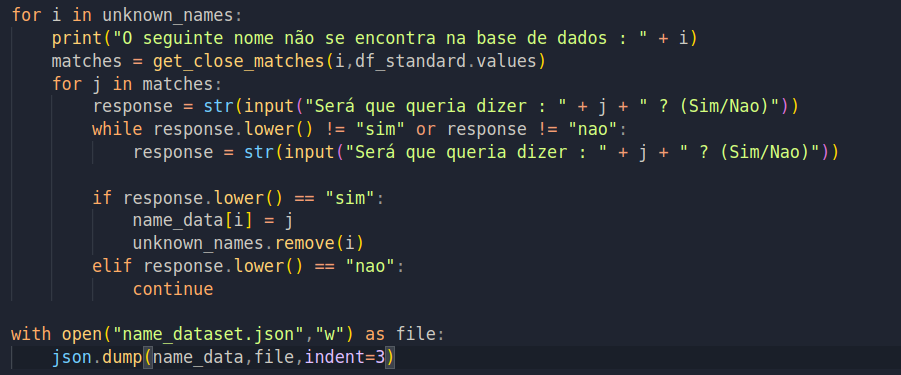
\includegraphics[width=14cm]{images/Screenshot3.png} \\[0.5cm]
% Se depois deste processo ainda existirem nomes desconhecidos é perguntado ao utilizador se pretende adicionar um novo nome á lista de nomes standard e ao dicionário de nomes, se sim então é lhe pedido que preêncha mais informações sobre o nome para que no futuro possam ser corrigidas linhas com esse nome.
% \vspace{0.5cm}

% 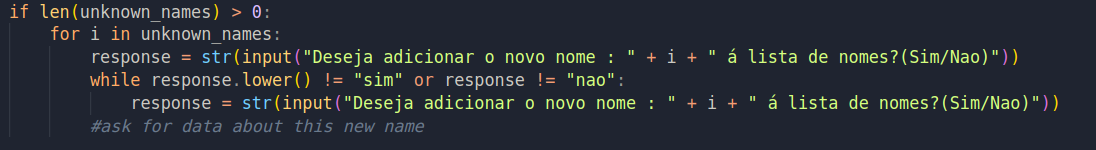
\includegraphics[width=14cm]{images/Screenshot4.png} \\[0.5cm]

% \subsection{Desafios e lições aprendidas}
% O maior desafio que estamos a enfrentar no momento centra-se precisamente no objectivo principal do projeto, a correção dos dados incorretos, devido ao tamanho dos dados fornecidos e á quantidade de erros cometidos nos mesmos o processo de associação dos nomes não pode ser feito manualmente já que demoraria imenso tempo, por isso como solução para este problema vamos utilizar métodos computacionais para determinar a correção de cada nome. 

% \newpage
% \bibliographystyle{plain}
% \bibliography{references}

\section{Testes e Resultados} \label{testes}

\subsection{Avaliação dos Dados e Mapeamento Inicial}

Durante a fase inicial, foi criada uma correspondência entre os nomes presentes nas tabelas fornecidas e os respetivos números de identificação. Nomes considerados variantes de um nome padrão foram identificados através de regras de similaridade e pré-processamento, nomeadamente através da limpeza e comparação por distância de Levenshtein. Com esta abordagem foi possível encontrar um nome padrão em cerca de 65\% dos casos. No entanto, falta de numeros de identificação e nomes mais complexos ou com um maior número de variações não eram corrigidos corretamente.

\subsection{Criação e Pós-processamento do Agrupamento}

Ao adicionar um novo nome ao processo de agrupamento, o seguinte procedimento é adotado:

\begin{enumerate}
    \item O nome é inicialmente inserido num grupo temporário, contendo apenas esse nome.
    
    \item Em seguida, são identificados os 1000 nomes mais semelhantes com base na métrica de similaridade. Apenas os nomes com pontuação superior a um limiar de pontuação correspondente a 0.81 são considerados para inclusão no grupo temporário.
    
    \item A inclusão desses nomes ao grupo temporário ocorre com as seguintes exceções:
    \begin{itemize}
        \item Caso o nome candidato já tenha sido adicionado anteriormente a um grupo, ele é ignorado.
        \item Caso o nome candidato pertença a um grupo originado a partir da base de verdade, também não é adicionado ao grupo temporário. Em vez disso, o índice desse nome e a sua respetiva similaridade são armazenados numa variável denominada \textit{best match}.
    \end{itemize}
    
    \item No fim do processo:
    \begin{itemize}
        \item Caso um \textit{best match} não tenha sido identificado, o grupo temporário é anexado como um novo grupo ao agrupamento existente.
        \item Caso um \textit{best match} tenha sido identificado, o grupo temporário não é adicionado como um novo agrupamento, mas sim utilizado para expandir o grupo base associado ao \textit{best match}.
    \end{itemize}
    \item Pos processamento: Explicado anteriomente no 5.2
\end{enumerate}
O limiar definido foi escolhido de acordo com um conjunto de testes realizados, dos quais se concluiu que este valor dava os melhores resultados de \textbf{F1-Score}, \textbf{Recall} e Precisão.
\newpage
\begin{figure}[h!]
    \centering
    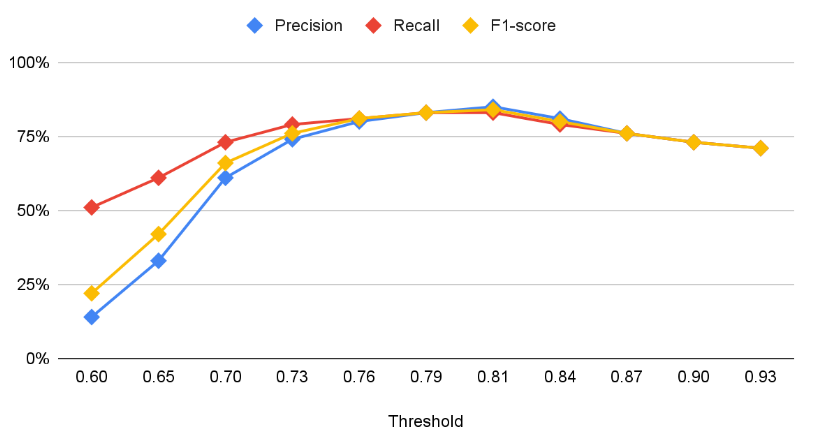
\includegraphics[width=0.8\textwidth]{images/threshold.png}
    \caption{Escolha do limiar}
    \label{fig:design}
\end{figure}
\noindent Métricas utilizadas para avaliar a qualidade dos agrupamentos

\begin{itemize}
    \item \textbf{Similaridade Intra-cluster}: considera a similaridade de um dado nome com os nomes pertencentes ao mesmo grupo.
    \item \textbf{Similaridade Inter-cluster}: considera a similaridade de um dado nome com os nomes de outros grupo.
\end{itemize}

\subsection{Avaliação de Precisão do Agrupamento}

Ao longo do presente relatório é destacado que o sistema desenvolvido permite opcionalmente a introdução de uma tabela de referência (\textit{standard}). Se uma tabela de referência for fornecida, a qualidade dos grupos de nomes aumenta, uma vez que os grupos iniciais são feitos com base nessa tabela. Ao utilizar 50\% desses dados, escolhidos aleatoriamente, é possível avaliar a qualidade do algoritmo verificando se os grupos criados são semelhantes aos restantes 50\%.

\begin{itemize}
    \item \textbf{Versão 1}: Agrupamento sem grupos base
    \item \textbf{Versão 2}: Agrupamento com 50\% dos grupos da base de verdade como base
\end{itemize}
\newpage
\begin{figure}[h!]
    \centering
    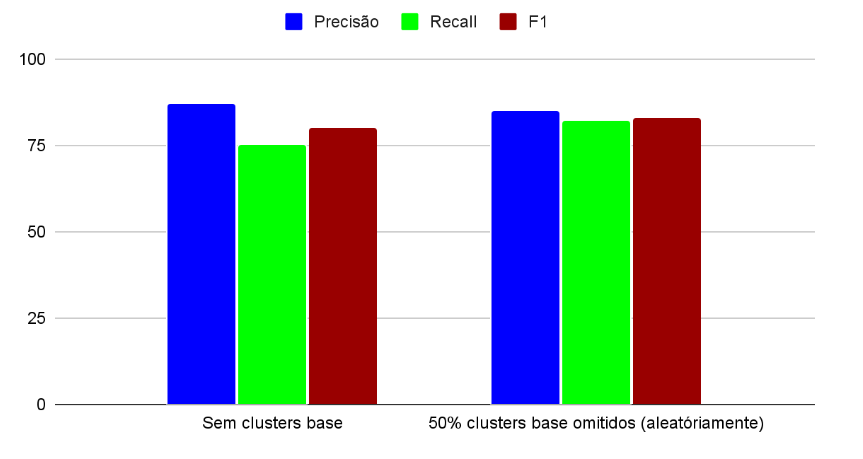
\includegraphics[width=0.8\textwidth]{images/clusterbase.png}
    \caption{Relevância da existência de grupos com origem na base de verdade no resultado final}
    \label{fig:design}
\end{figure}

\subsection{Criação do Mapa Final de Sinónimos}

Com base nos grupos, é criado automaticamente um mapa final de sinónimos que associa cada nome presente nas tabelas ao nome padrão correspondente, com base nos grupos obtidos. O mapa resultante gera uma nova coluna nas tabelas que associa a cada nome o seu nome padrão, de acordo com os grupos criados.

\subsection{Comparação de resultados com o método de MinHash}

Como referido anteriormente, na Secção~\ref{sec:MinHash}, a utilização da biblioteca \textbf{FAISS} resultou numa solução mais eficiente. Para além de uma redução significativa no tempo de execução, os resultados obtidos também apresentaram melhores resultados conforme as métricas utilizadas na avaliação do sistema.

% \begin{figure}[H]
%     \centering
%     \begin{minipage}{0.40\textwidth}
%         \centering
%         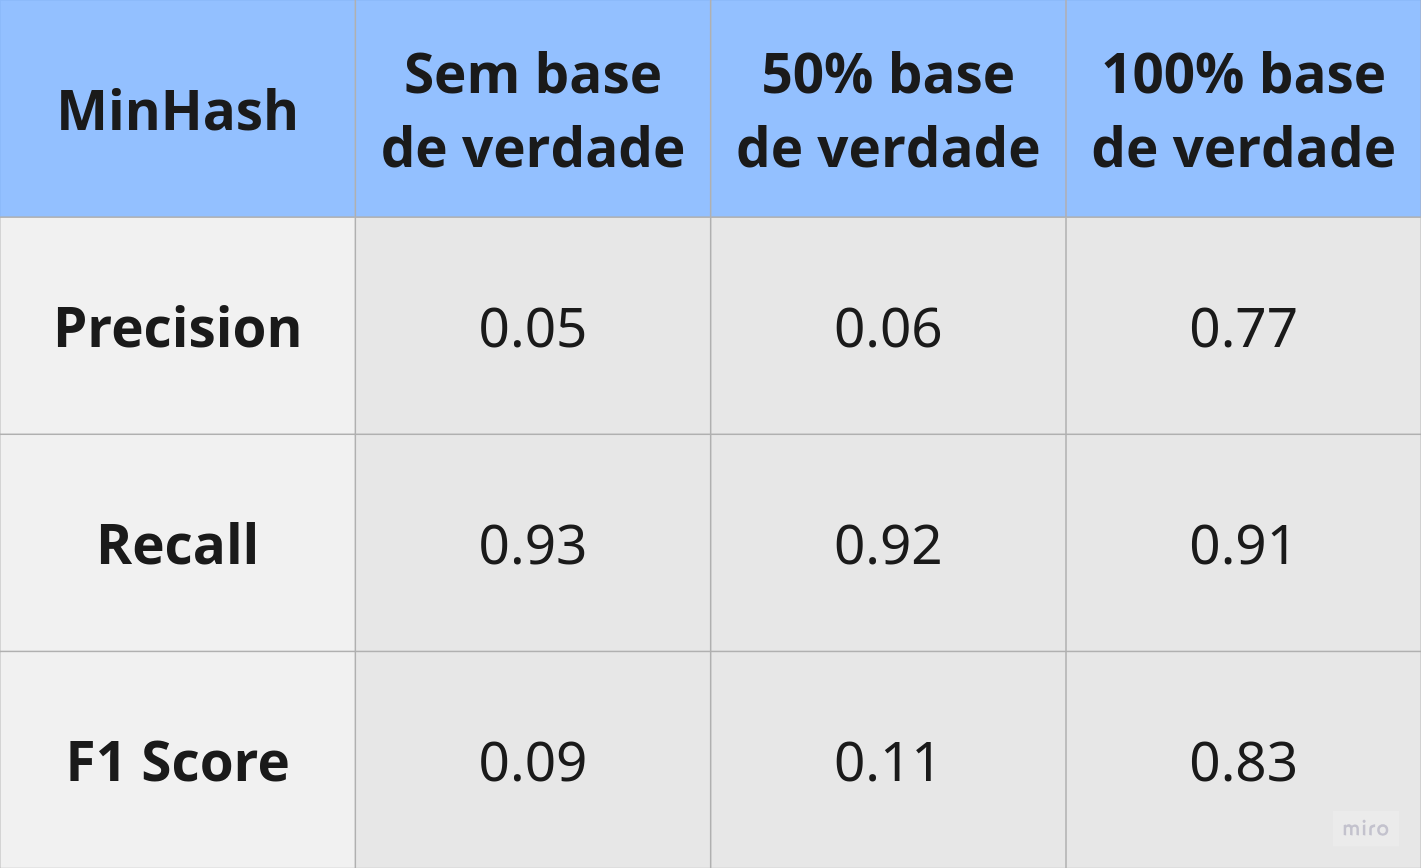
\includegraphics[height=4.5cm]{images/tableMinHash.png}
%         \caption*{(a) Resultados com MinHash}
%     \end{minipage}
%     \hfill
%     \begin{minipage}{0.40\textwidth}
%         \centering
%         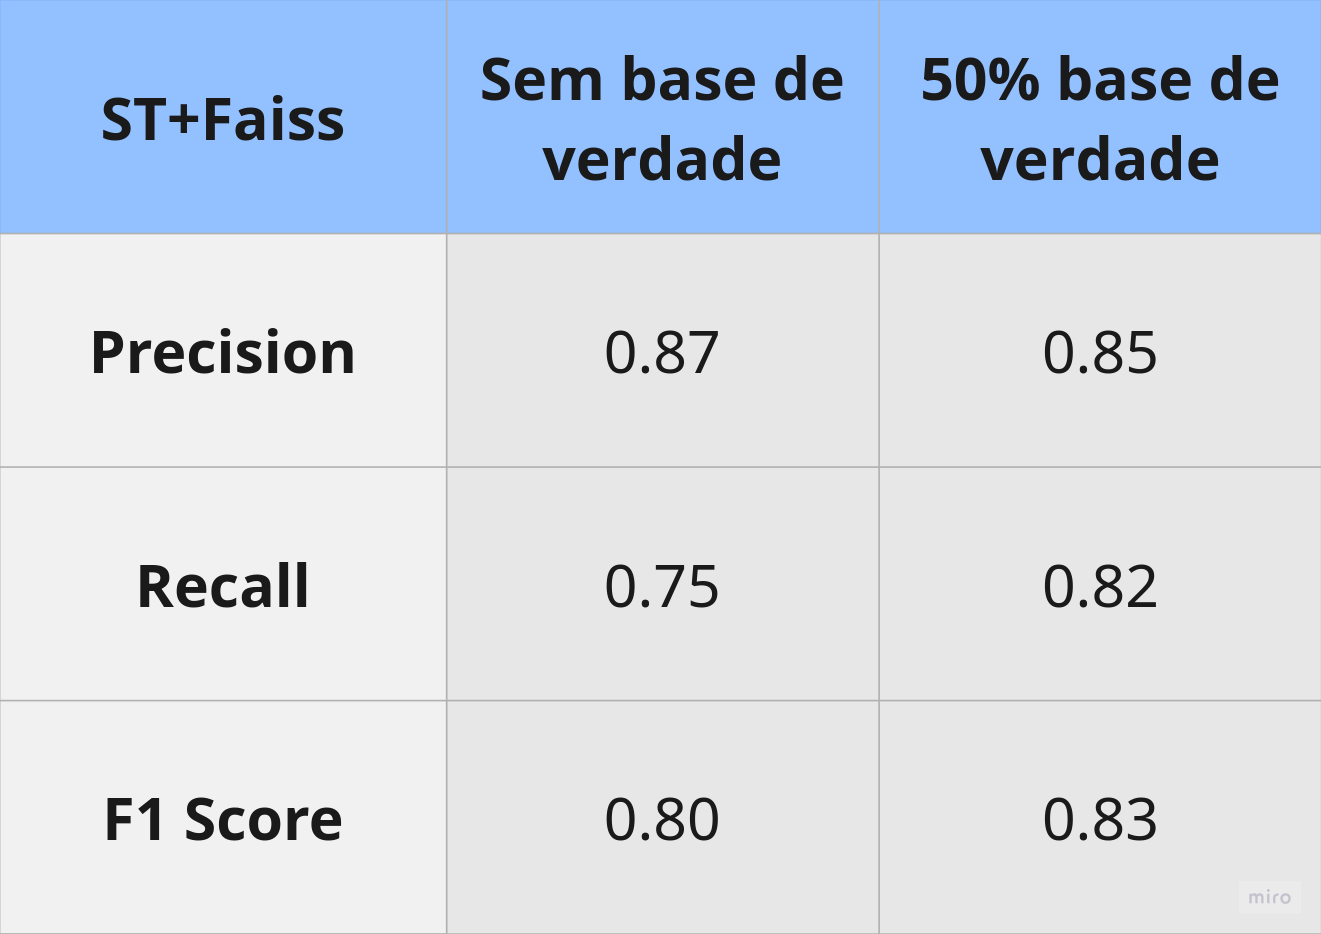
\includegraphics[height=4.5cm]{images/tableFaiss.png}
%         \caption*{(b) Resultados com a biblioteca FAISS}
%     \end{minipage}
% \end{figure}

\begin{figure}[h!]
    \centering
    \begin{minipage}{0.45\textwidth}  % minipage com 45% da largura total
        \centering
        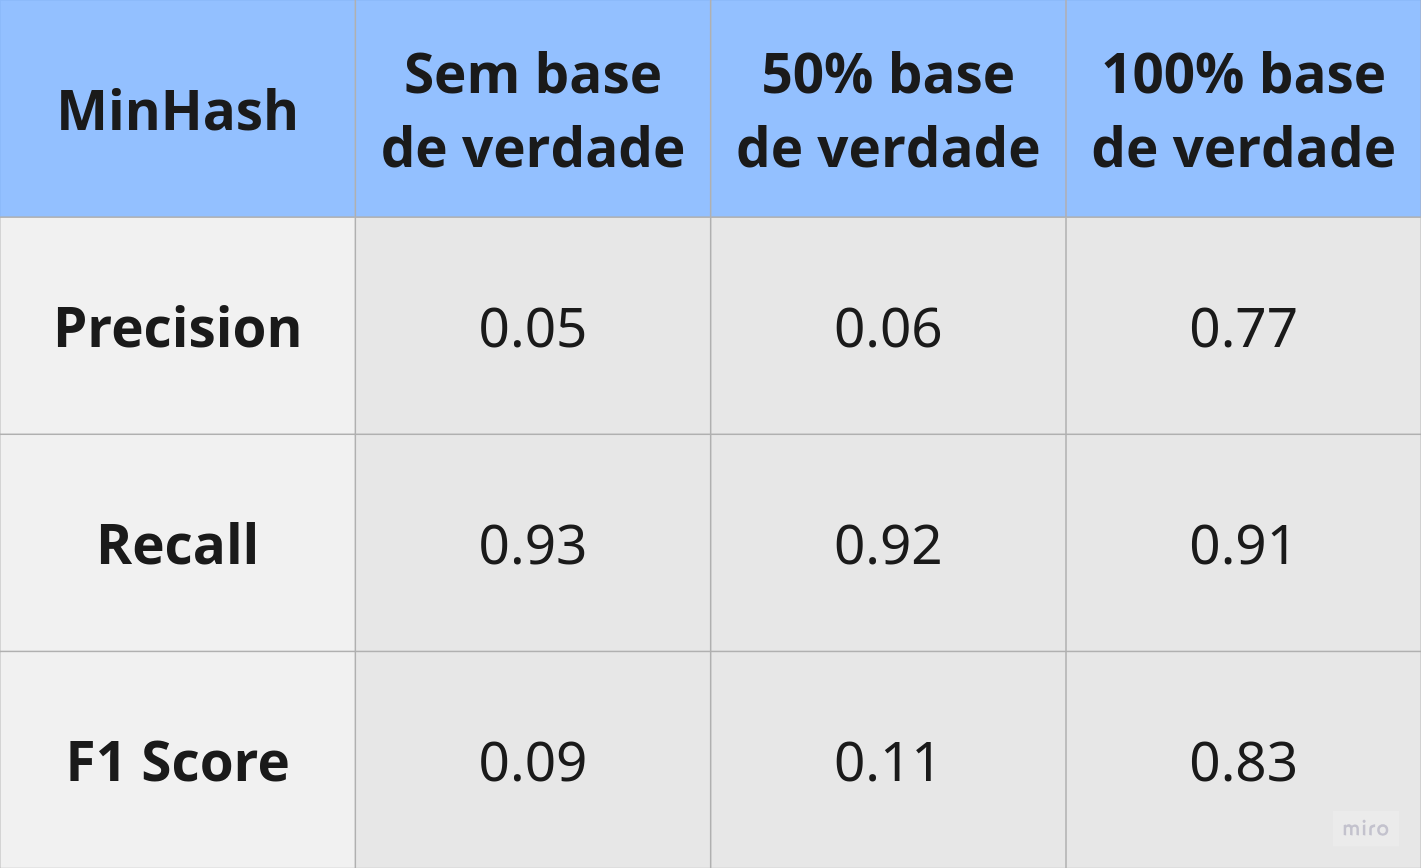
\includegraphics[width=\textwidth]{images/tableMinHash.png}
        \caption{Resultados MinHash}
    \end{minipage}
    \hfill
    \begin{minipage}{0.39\textwidth}
        \centering
        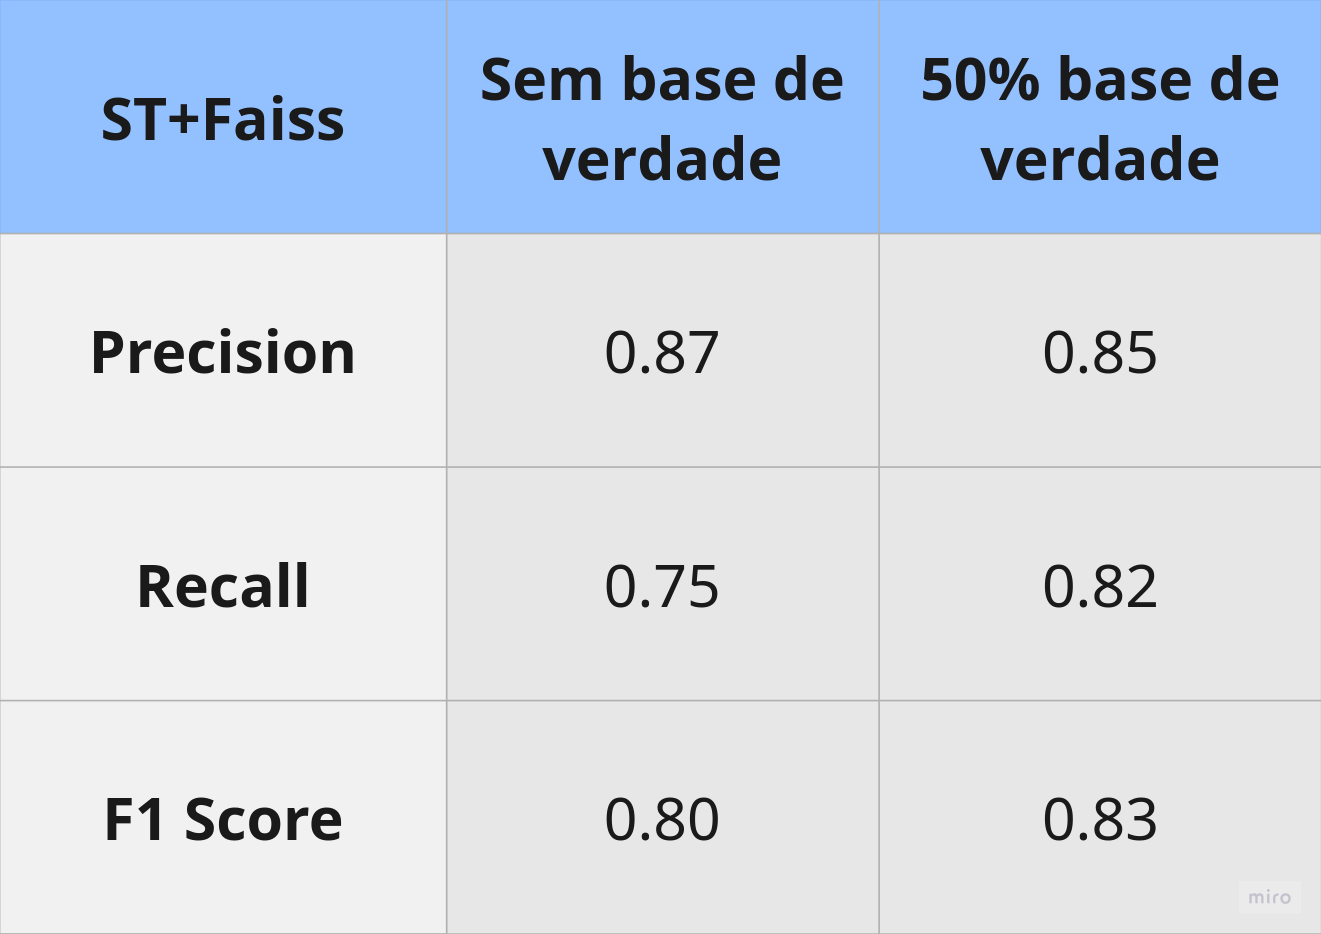
\includegraphics[width=\textwidth]{images/tableFaiss.png}
        \caption{Resultados ST+FAISS}
    \end{minipage}
\end{figure}

\newpage %adicionado porque cortava a section do texto logo no inicio, caso deixe de acontecer, remover
\section{Conclusão}

Em última análise, o grupo responsável pelo desenvolvimento do projeto, bem como o professor supervisor do mesmo, consideraram que o sistema desenvolvido cumpre os requisitos definidos na sua quase totalidade.
\\
Ao longo do desenvolvimento foram testadas várias soluções e, por fim, o grupo optou por uma solução que permite uma elevada percentagem de correção, bem como uma complexidade temporal reduzida.
O programa desenvolvido é flexível, nomeadamente pelo facto de ser totalmente opcional a introdução de uma tabela de referência.
\\
Posto isto, a solução desenvolvida pode ser facilmente adaptada a contextos reais, necessitando de eventuais ajustes dependendo do modo de utilização pretendido.
Além de cumprir os requisitos técnicos, o desenvolvimento do projeto proporcionou ao grupo um aprofundamento nas áreas do âmbito, especialmente a área de ciências de dados.

\newpage
\section{Bibliografia}
\bibliographystyle{plain}
\bibliography{referencias}

\end{document}